\section{信号叠加}
\label{sec:stack-files}
相关命令:\nameref{sss:addstack}、\nameref{sss:liststack}、
\nameref{sss:sumstack}、\nameref{sss:zerostack}

信号叠加可能是叠加地震波波形,也可能是叠加互相关函数等等,它是消除噪声,加强有效信号的常用手段。
SAC 通过提供一个子程序 Signal Stack Subprocess,简称 sss, 来实现。

\subsection{sss 的进入和退出}
在SAC中键入``!sss!''即可进入该子程序;在子程序中键入 \nameref{cmd:quitsub} 即可
退出子程序并回到主程序;也可键入 \nameref{cmd:quit} 直接从子程序中退出SAC。

\subsection{添加文件移除文件}

首先,需要让 SAC 读入要叠加的 SAC 文件。

\begin{SACCode}
SAC/SSS> ADDSTACK a WEIGHT 1 DELAY 20 SECONDS
\end{SACCode}

上面的例子是读入文件 a。
WEIGHT 1 是设置权重,即用 1 乘以 SAC 文件的每一个点的值,权重可以是 0 到 1 的数。
DELAY 20 SECONDS 是波形向后延迟 20 秒。

再看下面的例子。打开 SAC 后,读取了文件a。
然后,进入了 sss,用简写的方式添加了 a 和 b,其中文件 a 延迟 10s。
接着输入的 \nameref{sss:liststack} 命令不是列出当前路径的内容而是列出 sss 添加了哪些文件。
首先,我们可以看到有两个文件 a,这是因为之前在 sss 外读取了一次文件 a。
第二个 a 的 delayt 属性即 DELAY TIME 是 10。

\begin{SACCode}
SEISMIC ANALYSIS CODE [07/05/2015 (Version 101.6a)]
Copyright 1995 Regents of the University of California

SAC> r a
SAC> sss
Signal Stacking Subprocess.
SAC/SSS> as a delay 10 s
SAC/SSS> as b
SAC/SSS> ls

 filename  weight      delayt      delayn     delayvm   polarity   distance
                           delayti     delayni      begin       end
 a         1.000       0.000       0.000       0.000   NORMAL   -12345.000
                             0.000       0.000      10.000      14.000
 a         1.000       10.00       0.000       0.000   NORMAL   -12345.000
                             0.000       0.000      10.000      14.000
 b         1.000       0.000       0.000       0.000   NORMAL   -12345.000
                             0.000       0.000      20.000      24.000
 Time Window:       0.000       0.000
 Stack Velocity Model 1 OFF
 Stack Velocity Model 2 OFF
\end{SACCode}

\subsection{叠加文件}

本小节用两个脉冲函数做例子说明 sss 叠加文件。

首先,生成两个脉冲函数文件。

\begin{SACCode}
SEISMIC ANALYSIS CODE [07/05/2015 (Version 101.6a)]
Copyright 1995 Regents of the University of California
SAC> funcgen impulse npts 10 delta 1 begin 0
// 生成一个脉冲函数,数据点数 10 个,采样间隔 1s, 头段 b 为 0
SAC> w a
SAC> funcgen impulse npts 10 delta 1 begin 10
// 生成一个脉冲函数,数据点数 10 个,采样间隔 1s, 头段 b 为 10
SAC> w b
\end{SACCode}

上面的步骤生成了两个脉冲函数,我们现在尝试把它们叠加起来:

\begin{SACCode}
SAC> sss
 Signal Stacking Subprocess.
SAC/SSS> zs         // 清除之前添加的文件及各种设置
SAC/SSS> as a
SAC/SSS> as b
SAC/SSS> tw 0 19    // 确定时窗,必选设定
SAC/SSS> ss
\end{SACCode}

\begin{figure}[H]
\centering
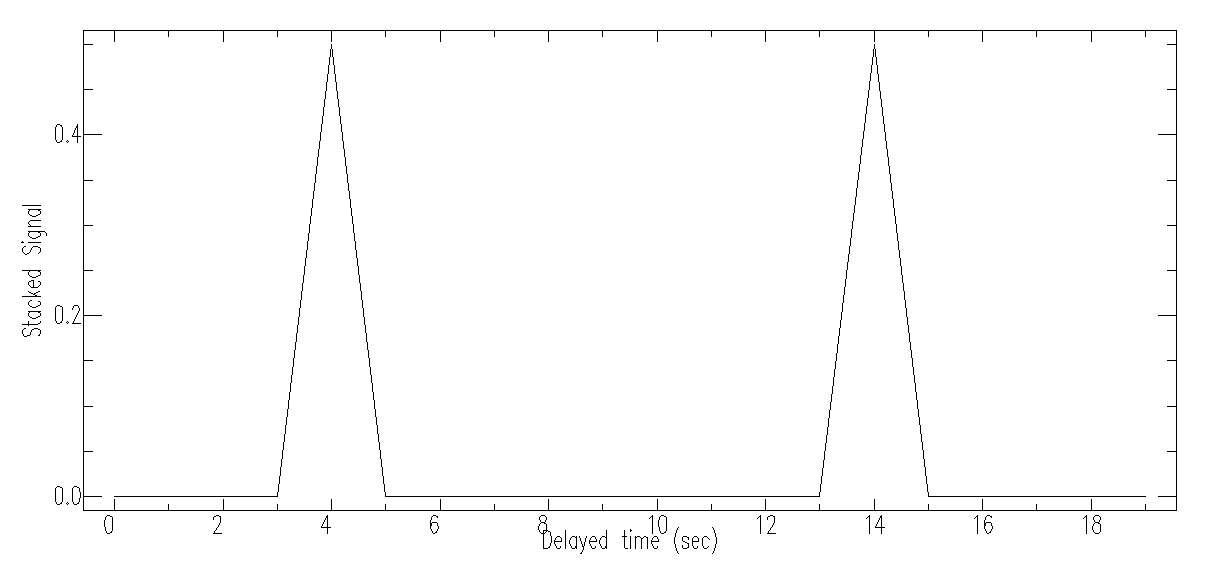
\includegraphics[width=0.8\textwidth]{stack-without-delay}
\caption{不做动校正的叠加}
\label{fig:filter-waveform}
\end{figure}

ss 就是叠加命令。执行后,SAC 会自动弹出叠加后的波形图。我们可以看到两个脉冲信号。
叠加的方式需要理解到两点:一是波形是按相对时刻对齐的。
二是叠加默认会均一化,所以看到最到振幅只有 0.5。
下面我们尝试把 a 和 b 叠加起来,并做动校正让脉冲信号重合,并且振幅就是简单的求和使其等于 2。

\begin{SACCode}
SAC/SSS> zs
SAC/SSS> as a delay 10 s
SAC/SSS> as b
SAC/SSS> tw 0 19
SAC/SSS> ss n off
\end{SACCode}

结果如图:

\begin{figure}[H]
\centering
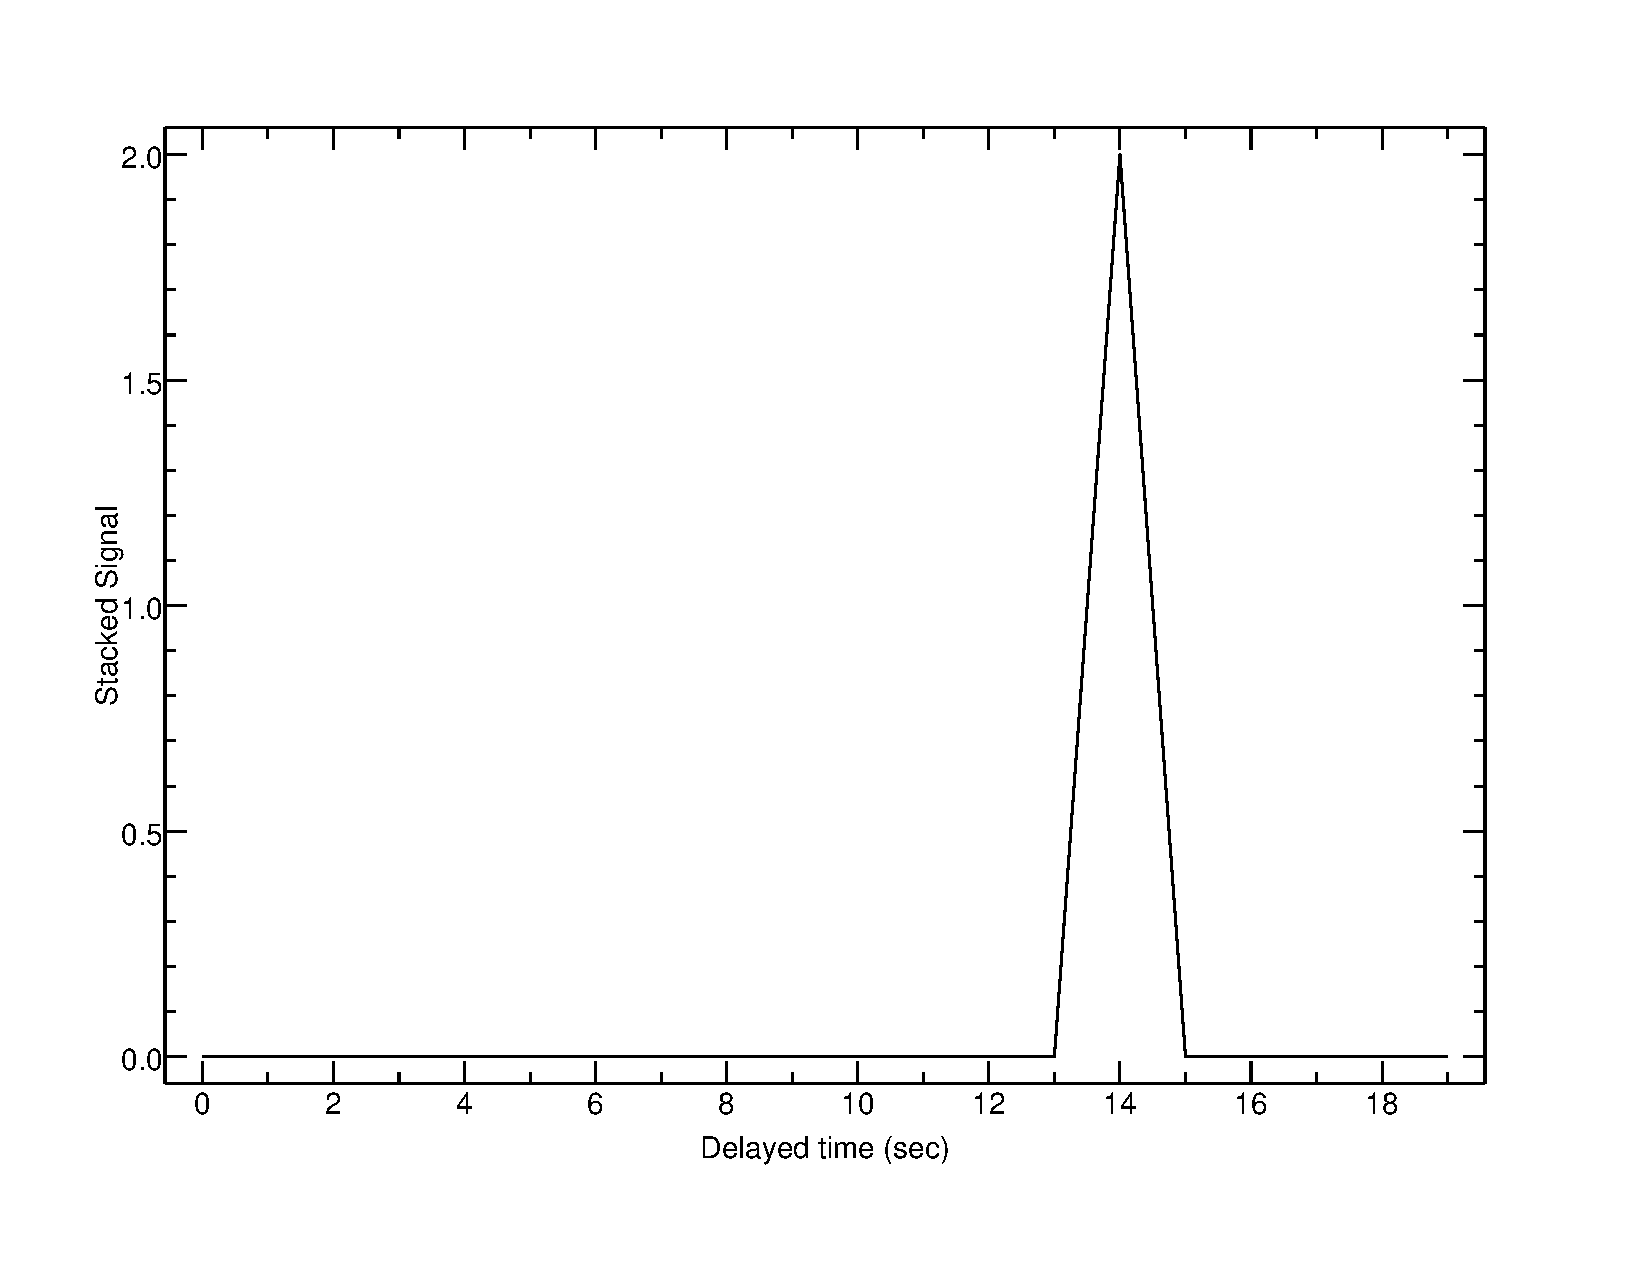
\includegraphics[width=0.8\textwidth]{stack-with-delay}
\caption{做动校正的叠加}
\label{fig:filter-waveform}
\end{figure}
